%!TEX root = ../dissertation.tex

\chapter{Background}
\label{chapter:background}
This chapter presents the background necessary to understand the area of the problem to be solved.
First section reviews the relevant related work to solve the challenges of converging the Internet
of Things and Utility Computing. The following sections present a description of the concepts
that composes the basis of our work.

% Cloud computing concepts and tools
\section{Cloud computing concepts and tools}
\label{sub:cloud_concepts_tools}
Recently a lot of research and effort has been dedicated to solve these existing problems. In this
section we will present a summary of the most relevant work that relates to the convergence of the
Internet of Things with the Utility Computing in the cloud:

% Smart Place Deployment
\subsection{Smart Place Deployment}
\label{sub:smart_place_deployment}
As referred in Section~\ref{section:challenges}, current \gls{IoT} solutions are delivered in a physical
and isolated manner, which makes its service delivery model an inefficient and unscalable process.
In order to turn the service delivery of \gls{IoT} solutions more efficient and scalable, cloud service
delivery models are being developed based on the existing layers of the cloud architecture \cite{zhang2010cloud}:

% Cloud architecture layers
\begin{itemize}
  % IaaS
  \item\textit{\gls{IaaS}} refers to the provisioning of infrastructure resources on-demand - e.g.
  \glspl{VM}, storage and network.
  % PaaS
  \item\textit{\gls{PaaS}} refers to providing platform layer resources such as operating system support
  and software development frameworks.
  % SaaS
  \item\textit{\gls{SaaS}} refers to providing on demand application over the Internet.
\end{itemize}

% Soldatos
\subparagraph{Soldatos} et al. \cite{soldatos2012convergence} presented the idea of converging the IoT
and the utility computing in the cloud. The proposed architecture is the core concept of the OpenIoT
Project\footnote{\url{http://openiot.eu}}, and is based on CoAP \cite{shelby2014constrained} and linked data.
The cloud is used at infrastructure level, which allows to measure the utility of the services provided
by inter-connected objects.
% Distefano
\subparagraph{Distefano} et al. \cite{distefano2012enabling} proposed a conceptual architecture by
mapping various elements in both cloud and IoT to the three layers of the cloud architecture (\gls{IaaS},
\gls{PaaS} and \gls{SaaS}). In this proposal IoT resources are provided voluntarily by their owners,
while management functions - such as node management and policy enforcement - are viewed as peer
functions of cloud infrastructure management. A \gls{PaaS} module is responsible to mashup IoT and
cloud infrastructure (\gls{IaaS}) resources for applications, which are delivered to the clients
through \gls{SaaS}.
% CloudThings
\subparagraph{CloudThings} \cite{zhou2013cloudthings} is an architecture that uses a common
approach to integrate Internet of Things and Cloud Computing. The proposed architecture is an online
platform which accommodates \gls{IaaS}, \gls{PaaS}, \gls{SaaS} and allows system integrators and
solution providers to leverage the complete application infrastructure for developing, operating
and composing applications and services.
% IoT PaaS
\subparagraph{Li} et. al \cite{li2013efficient} proposed IoT PaaS, a cloud platform that supports
scalable IoT service delivery. Solution providers are able to deliver new solutions by leveraging
computing resources and platform services - domain mediation, application context management, etc.
- to the cloud. The proposed architecture aims to enable virtual vertical service delivery, for that
it has a multi-tenant nature which is designed to help at the isolation of the environments of
different solutions.\\

Although great progress was achieved regarding the improvement of service delivery for \gls{IoT}
solutions, most of the work still are in a conceptual stage. What is certain is that cloud service
delivery models will be the basis for the service delivery models of \gls{IoT} solutions.

% Data Storage Performance
\subsection{Data Storage Performace}
\label{sub:data_storage}
Since that data storage and retrieval in the cloud had specific requirements, cloud providers started
to implement their own solutions.

\subparagraph{Google Big Table, Facebook Cassandra and  Amazon Dynamo} \cite{chang2008bigtable} \cite{lakshman2010cassandra}
\cite{decandia2007dynamo} are key-value stores - \gls{NoSQL} databases - that have the ability to horizontally scale - i.e,
distribute both data and load of simple operations through many servers - but it has a weaker consistency
model than the ACID transactions of most \glspl{RDBMS} systems \cite{cattell2011scalable}.

\subparagraph{\gls{PIQL}} \cite{armbrust2010piql} is a SQL-like API built to run on top of existing
performance predictable key-value stores, that provides many of the benefits of using a traditional
\gls{RDBMS}, such as the ability to express the queries in a declarative way, automatic data
parallelism, physical data independence and automatic index selection and maintenance, all while
maintaining the low latency guarantees on application performance that come from the underlying
key-value store.\\

Recently, some progress has been reached as regards scalable storage for \gls{RDBMS} systems. Although most
of the works are still in development, it is possible to highlight some solutions that are in a more
mature state.

\subparagraph{MySQL Cluster} \cite{ronstrom2004mysql} is an in-memory clustered distributed \gls{RDBMS}.
Compared with the basic MySQL implementation it works by replacing the InnoDB engine with the NDB - a proprietary
distributed layer from MySQL. MySQL Cluster is built on top of a shared-nothing architecture and includes
features such as failover, node recovery, synchronous data replication and no single point of failure.
MySQL Cluster seesm to be the solution that scales to more nodes than other \gls{RDBMS} - 48 is the limit.
However, it was reported that after scaling up to a few dozen nodes it starts to running into
bottlenecks \cite{bunch2010evaluation}.

\subparagraph{VoltDB} \cite{stonebraker2013voltdb} is a \gls{RDBMS} designed for performance and scalability.
VoltDB assumes a multi-node cluster architecture where the tables are partitioned over multiple servers.
Tables can be replicated over servers - e.g. for fast access to data - shards are always replicated -
to recovery the data in case of a node crash - and database snapshots are supported. Currently some
features still are missing - online schema changes are limited and asynchronous \gls{WAN} replication and
recovery are not yet implemented - but in its current implementation VoltDB already presents some
features that improves the performance of SQL execution. As result, the number of nodes that are
needed to support a given application load can be reduced in a significant way.

% Containers
\subsection{Containers}
\label{sub:containers}
Containers are a virtualization technique that is performed at the \gls{OS} level, different of
hypervisor-based solutions - e.g. \glspl{VM} - where the virtualization is performed at the hardware-level.
In a \gls{OS} level virtualization, all guests share the same operating system as the base machine \cite{matthews2007quantifying}.
Although the effect of both types of virtualization are similar, unlike the hypervisor-based virtualization
an \gls{OS} level virtualization does not provide the ability to run multiple \glspl{VM} with different
operating systems on the same physical machine. However, \gls{OS} level virtualization provides significant
benefits when compared to hypervisor-based solutions. Containers are small, they have low memory and
\gls{CPU} overhead, they also are portable between different virtualization environments \cite{soltesz2007container}.\\

\subsubsection{Docker Platform}
\label{subs:docker_platform}
Docker\footnote{\url{https://www.docker.com/}} is an open source project to pack, ship and run any application as
a lightweight container. Docker is based on \gls{LXC}, which are hardware-agnostic and platform-agnostic,
meaning that these containers can run anywhere\footnote{Initially, Docker required that the physical
machine where the containers will be created is running a Linux kernel. Currently, Microsoft
launched Windows Server Containers, an \gls{OS} level virtualization mechanism where it is possible to
perform the management of containers through Docker.}, from a laptop to a cloud instance. Another
benefit that Docker platform provides is the Docker Hub\footnote{\url{https://hub.docker.com/}} service,
a public repository that stores Docker images that are used to create the containers.

% Configuration Management Tools
\subsection{Configuration Management Tools}
\label{sub:cm_tools}
\gls{CM} tools are software management tools that allows to automate and specify the deployment of an
application. Usually, users describe the system resources and their desired state and the \gls{CM}
tool is responsible to enforce the desired state. For instance, \gls{CM} tools allows the automation
of the provisioning of physical and virtual machines, perform dependency management of software
components and to perform the automation of management tasks.\\

Currently, there are several solutions to perform configuration management of software, where the
most relevant are Chef\footnote{\url{https://www.chef.io/}}, Puppet\footnote{\url{https://puppetlabs.com/}},
Ansible\footnote{\url{http://www.ansible.com/}} and Salt\footnote{\url{http://saltstack.com/}}. The main difference
between these tools is that some of the them are more oriented to developers, which is the case of Chef and
Puppet that requires some programming experience to be used, while others are more oriented to system
administrators, which is the case of Ansible and Salt.

% Chef
\subsubsection{Chef}
\label{subs:chef}
Chef is a configuration management tool that allows to describe the infrastructure as code.
In that way it is possible to automate how the infrastructure is built, deployed and managed.
Chef architecture is composed of the Chef Server - that stores the recipes and other configuration
data - and the Chef Client - that is installed in each server, \gls{VM} or container, i.e, the nodes that
are managed with Chef. The Chef client periodically pulls Chef server latest policy and state of the
network, and if anything on the node is out of date, the client update its state in order to be
consistent with the latest policy.\\

The tool was built from the ground with up the cloud infrastructure in mind. With Chef, it is possible
to dynamically provision and deprovision the application infrastructure on demand to keep up with
peaks in usage and track. For instance, the \textit{knife} command has a plugin for provisioning cloud
resources across several cloud providers - \gls{AWS}\footnote{\url{https://aws.amazon.com/}}, Google
Compute Engine\footnote{\url{https://cloud.google.com/compute/}} and Openstack\footnote{\url{https://www.openstack.org/}}.\\

% Fog Computing
\section{Fog computing for low latency responses}
\label{sec:fog_computing}
The Fog Computing \cite{bonomi2012fog} is a platform that aims to bring the cloud close to the ``edge
of the Network''. By bringing the cloud close to the ground - hence the fog analogy - the Fog will be
able to meet the requirements of several applications that the traditional clouds are not able to
accomplish. The most notable case is the Internet of Things, that requires mobility support,
geo-distribution in addition to location awareness and low latency. The Fog aims to achieve that by
virtualizing the computing, storage and network services between end devices and the
traditional data centers in the cloud.\\

% Fog Computing Infrastructure
\begin{figure}[ht!]
  \centering
  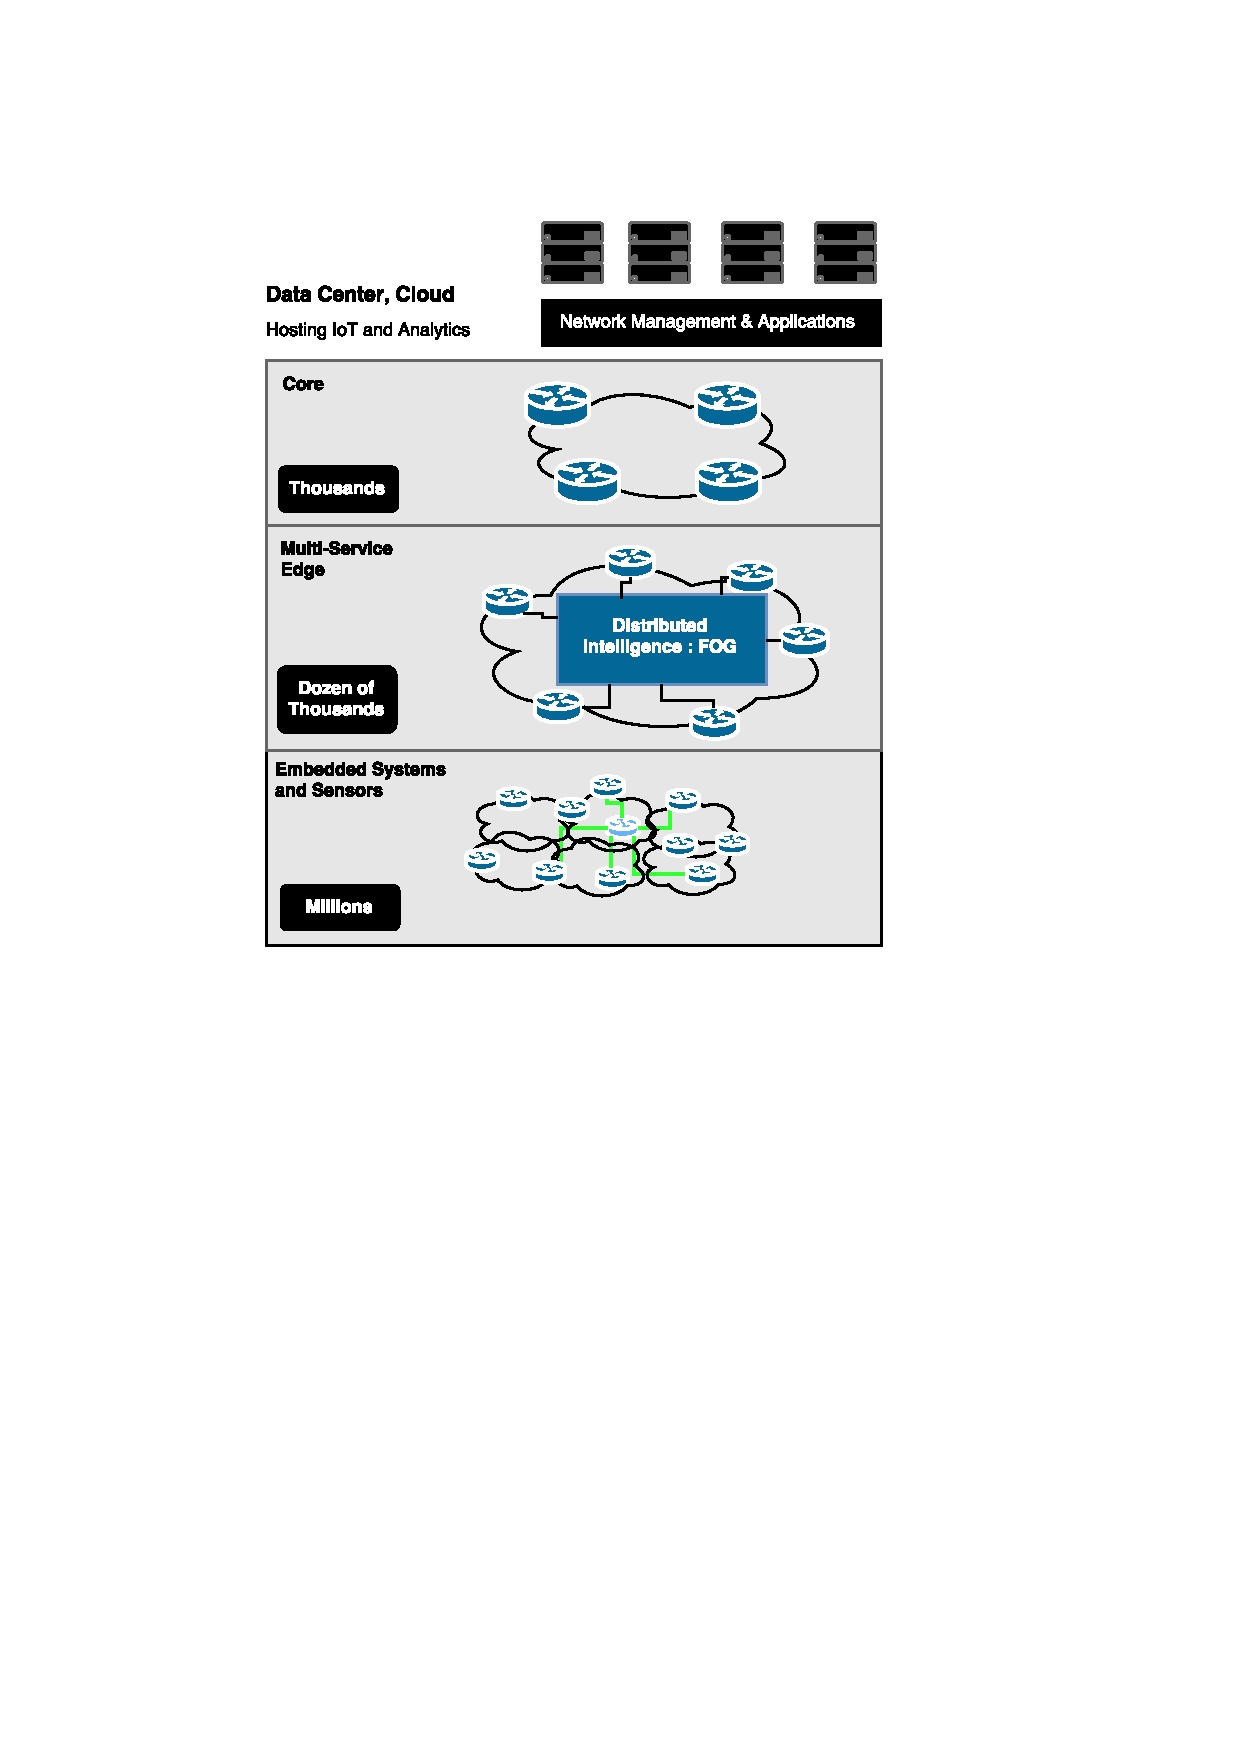
\includegraphics[width=.9\textwidth]{./images/fog_architecture}
  \caption[IoT and Fog Computing.]{The Internet of Things and Fog Computing (Bonomi et. al (2012)).}
  \label{fig:fog_architecture}
\end{figure}

Bonomi et. al \cite{bonomi2012fog} presents the architecture of a Fog Computing platform. As illustrated
in Figure~\cite{bonomi2012fog} the distributed infrastructure of the Fog is composed of heterogeneous
resources that must be managed in a distributed way: the infrastructure comprising of several players,
covering from data centers, core of the network, edge of the network and end devices. The \textit{Embedded Systems and Sensors}
is the lowest layer of the Fog and it is responsible to perform \gls{M2M} interaction. It collects and
process the data from the sensors, issues commands to the actuators and also filters the data that
is locally consumed and sent to the higher layers. The \textit{Multi-Service Edge} and \textit{Core}
layers are responsible for performing visualization and reporting - e.g. \gls{H2M} interaction -
as well to deal with systems and processes (\gls{M2M}).\\

Since the interaction time between the different layers can range from seconds - e.g. low-latency real-time
analytics - to days - transactional analytics - the Fog must support several types of storage, from
ephemeral storage at the lowest layers to semi-permanent at the highest layer. It is important to point
that the higher is the tier, the geographical coverage is wider and the time scale is larger \cite{bonomi2014fog}.
The global coverage is given by the Cloud, which acts as a central repository for the persistent data
and that is used to perform business analytics.

\section{Internet of Things stack example: EPC Framework}
\label{sec:iot_stack}
The \gls{RFID} middleware is the component of a \gls{RFID} system that sits between the low level
components - e.g. readers and tags - and the business client application - e.g. \gls{ERP} systems.
The next paragraphs describes the EPCglobal, a framework that provides standardized interfaces that
isolates hardware vendors from business applications, and Fosstrak, a open-source \gls{RFID}
middleware platform that implements the GS1 \gls{EPC} Network standards.

% GS1 EPC Network
\subsection{GS1 EPCglobal Architecture}
\label{subs:epc_network}
GS1\footnote{\url{http://www.gs1.org}} is an organization that is responsible for the development and maintenance of standards for
supply chain. One of the standards developed by GS1 is the \gls{EPC}, which is an unique serial identifier
for \gls{RFID} tags. GS1's subsidiary EPCglobal Inc.\footnote{\url{http://www.gs1.org/epcglobal}} created
the EPCglobal Architecture Framework, that currently is the standard for \gls{RFID} platforms.
Figure~\ref{fig:epc_architecture} presents a high-level architecture of the EPCglobal framework
that shows its main interfaces and roles.\\

% EPC Architecture
\begin{figure}[ht!]
  \centering
  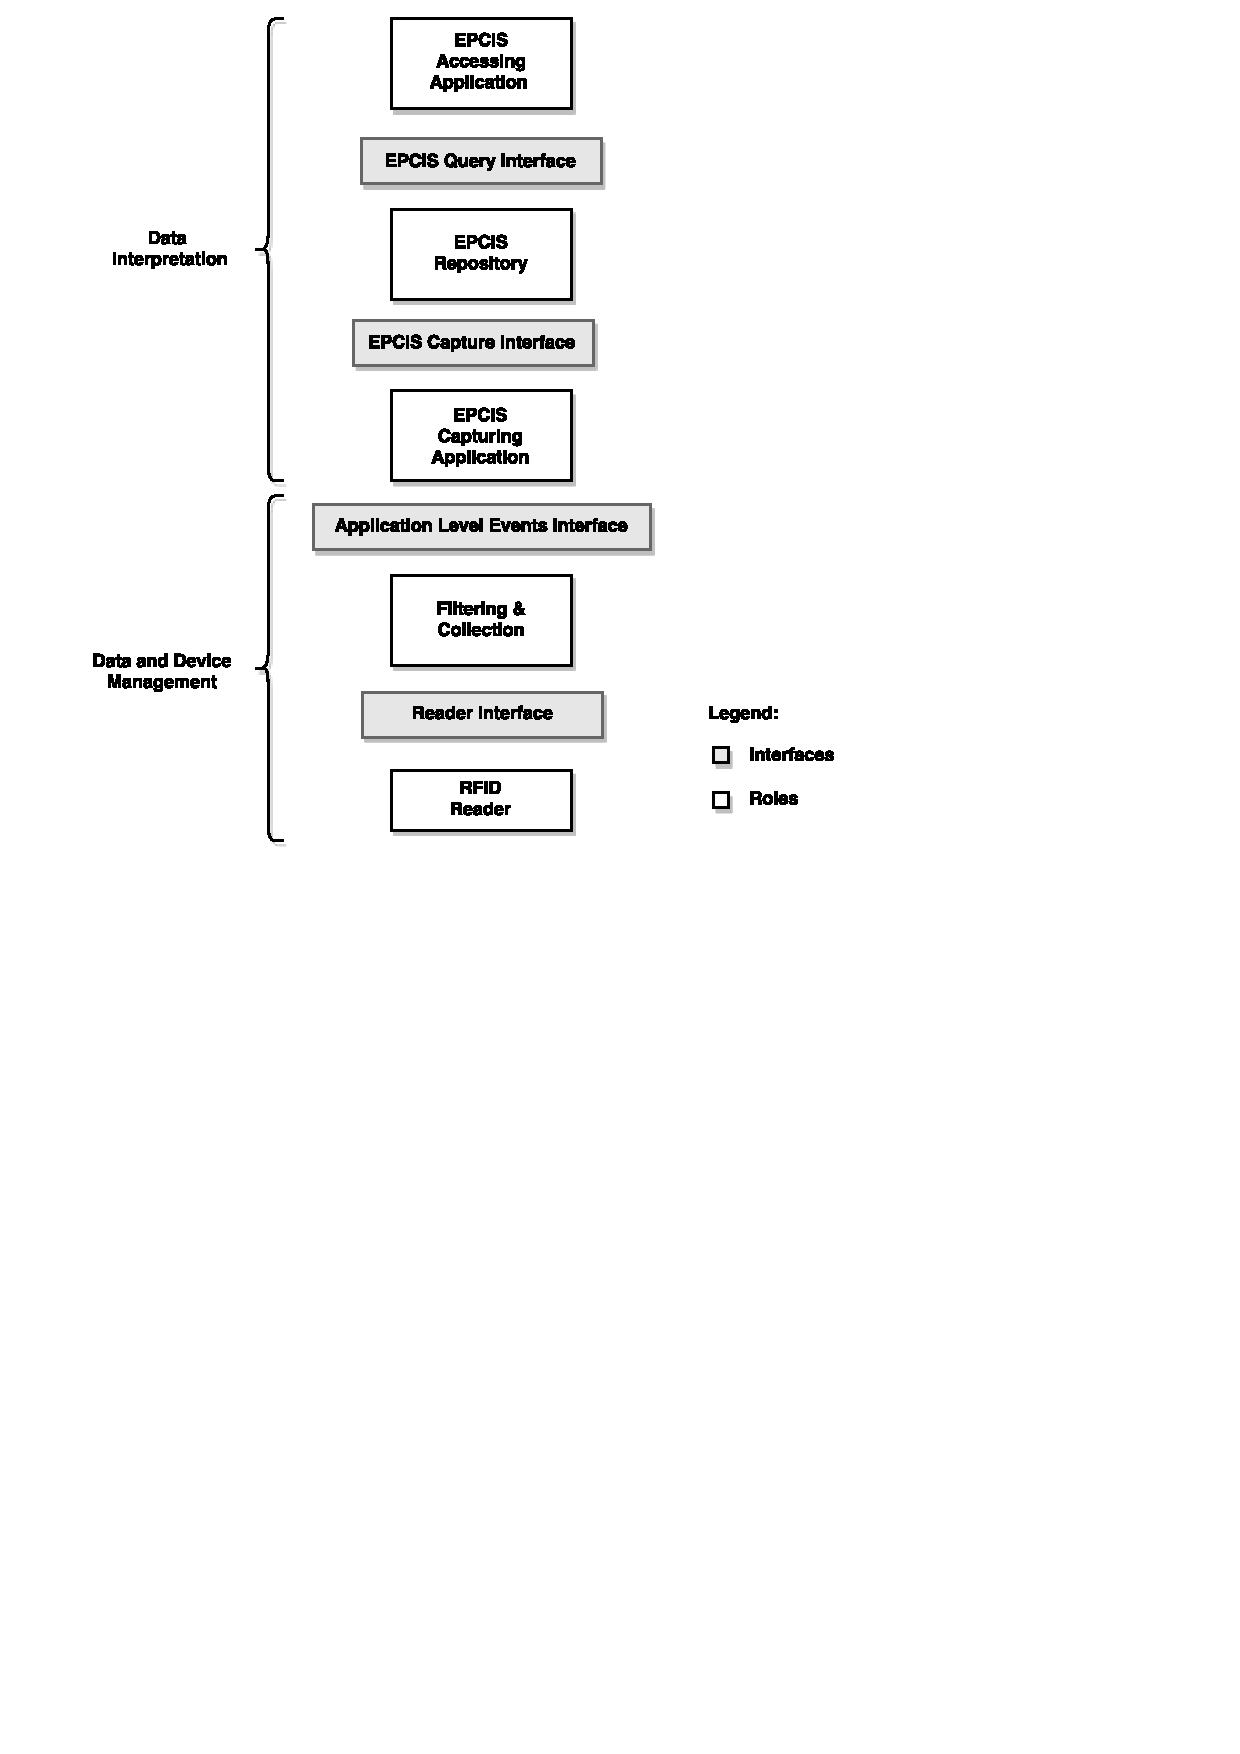
\includegraphics[width=.8\textwidth]{./images/EPCGlobal_architecture}
  \caption[EPCGlobal Architecture Framework.]{GS1 EPCGlobal Architecture Framework.}
  \label{fig:epc_architecture}
\end{figure}

The framework\footnote{For more information about the standards of the EPCglobal Framework, the
full documentation is available at \url{http://www.gs1.org/gs1-architecture}} has a
set of standardized interfaces that enables the interchange of information between entities. In the
context of our work, the most relevant components of the framework architecture are:

% EPC Architecture components
\begin{itemize}
  % Reader Interface
  \item \textit{Reader Interface} provides the interfaces that must be implemented by the \gls{RFID} readers.
  The \gls{LLRP} standard provides interfaces that allows the control of all the aspects of \gls{RFID}
  reader operation.
  % Filtering & Collection
  \item \textit{Filtering \& Collection} is the module that coordinates the \gls{RFID} readers that are in the
  same physical space and also abstracts the readers from the upper layers. It allows the execution of
  read and write operations on tags. Furthermore, it is responsible for filtering, aggregating and
  grouping the raw tag data when requested.
  % Filtering & Collection Interface
  \item \textit{\gls{ALE} Interface} defines the control and delivery of filtered and collected data from the
  Filtering \&  Collection module to the \gls{EPCIS} Capturing Application. The \glspl{ALE} are a selection of
  the events that are meaningful for the client applications.
  % EPCIS Capture Application
  \item \textit{EPCIS Capture Application} supervises the operation of the lower EPC layers, and provides
  business context based on information involved in the execution of a particular step of a business
  process.
  % EPCIS Repository
  \item \textit{EPCIS Repository} is the module where all the business events generated by the
  EPCIS Capturing Applications are stored to later be accessed by the EPCIS Accessing Application.
  The EPCIS Query Interface defines how client applications can retrieve information from the repository.
\end{itemize}

% Fosstrak
\subsection{Fosstrak Platform}
\label{sub:fosstrak}
The Free and Open Source Software for Track and Trace (Fosstrak) is an EPCglobal Network compliant
\gls{RFID} software platform that was developed by Floerkemeier et. al \cite{floerkemeier2007rfid}.
Figure~\ref{fig:fosstrak_architecture} presents the architecture of the Fosstrak platform.

% Fosstrak Architecture
\begin{figure}[ht!]
  \centering
  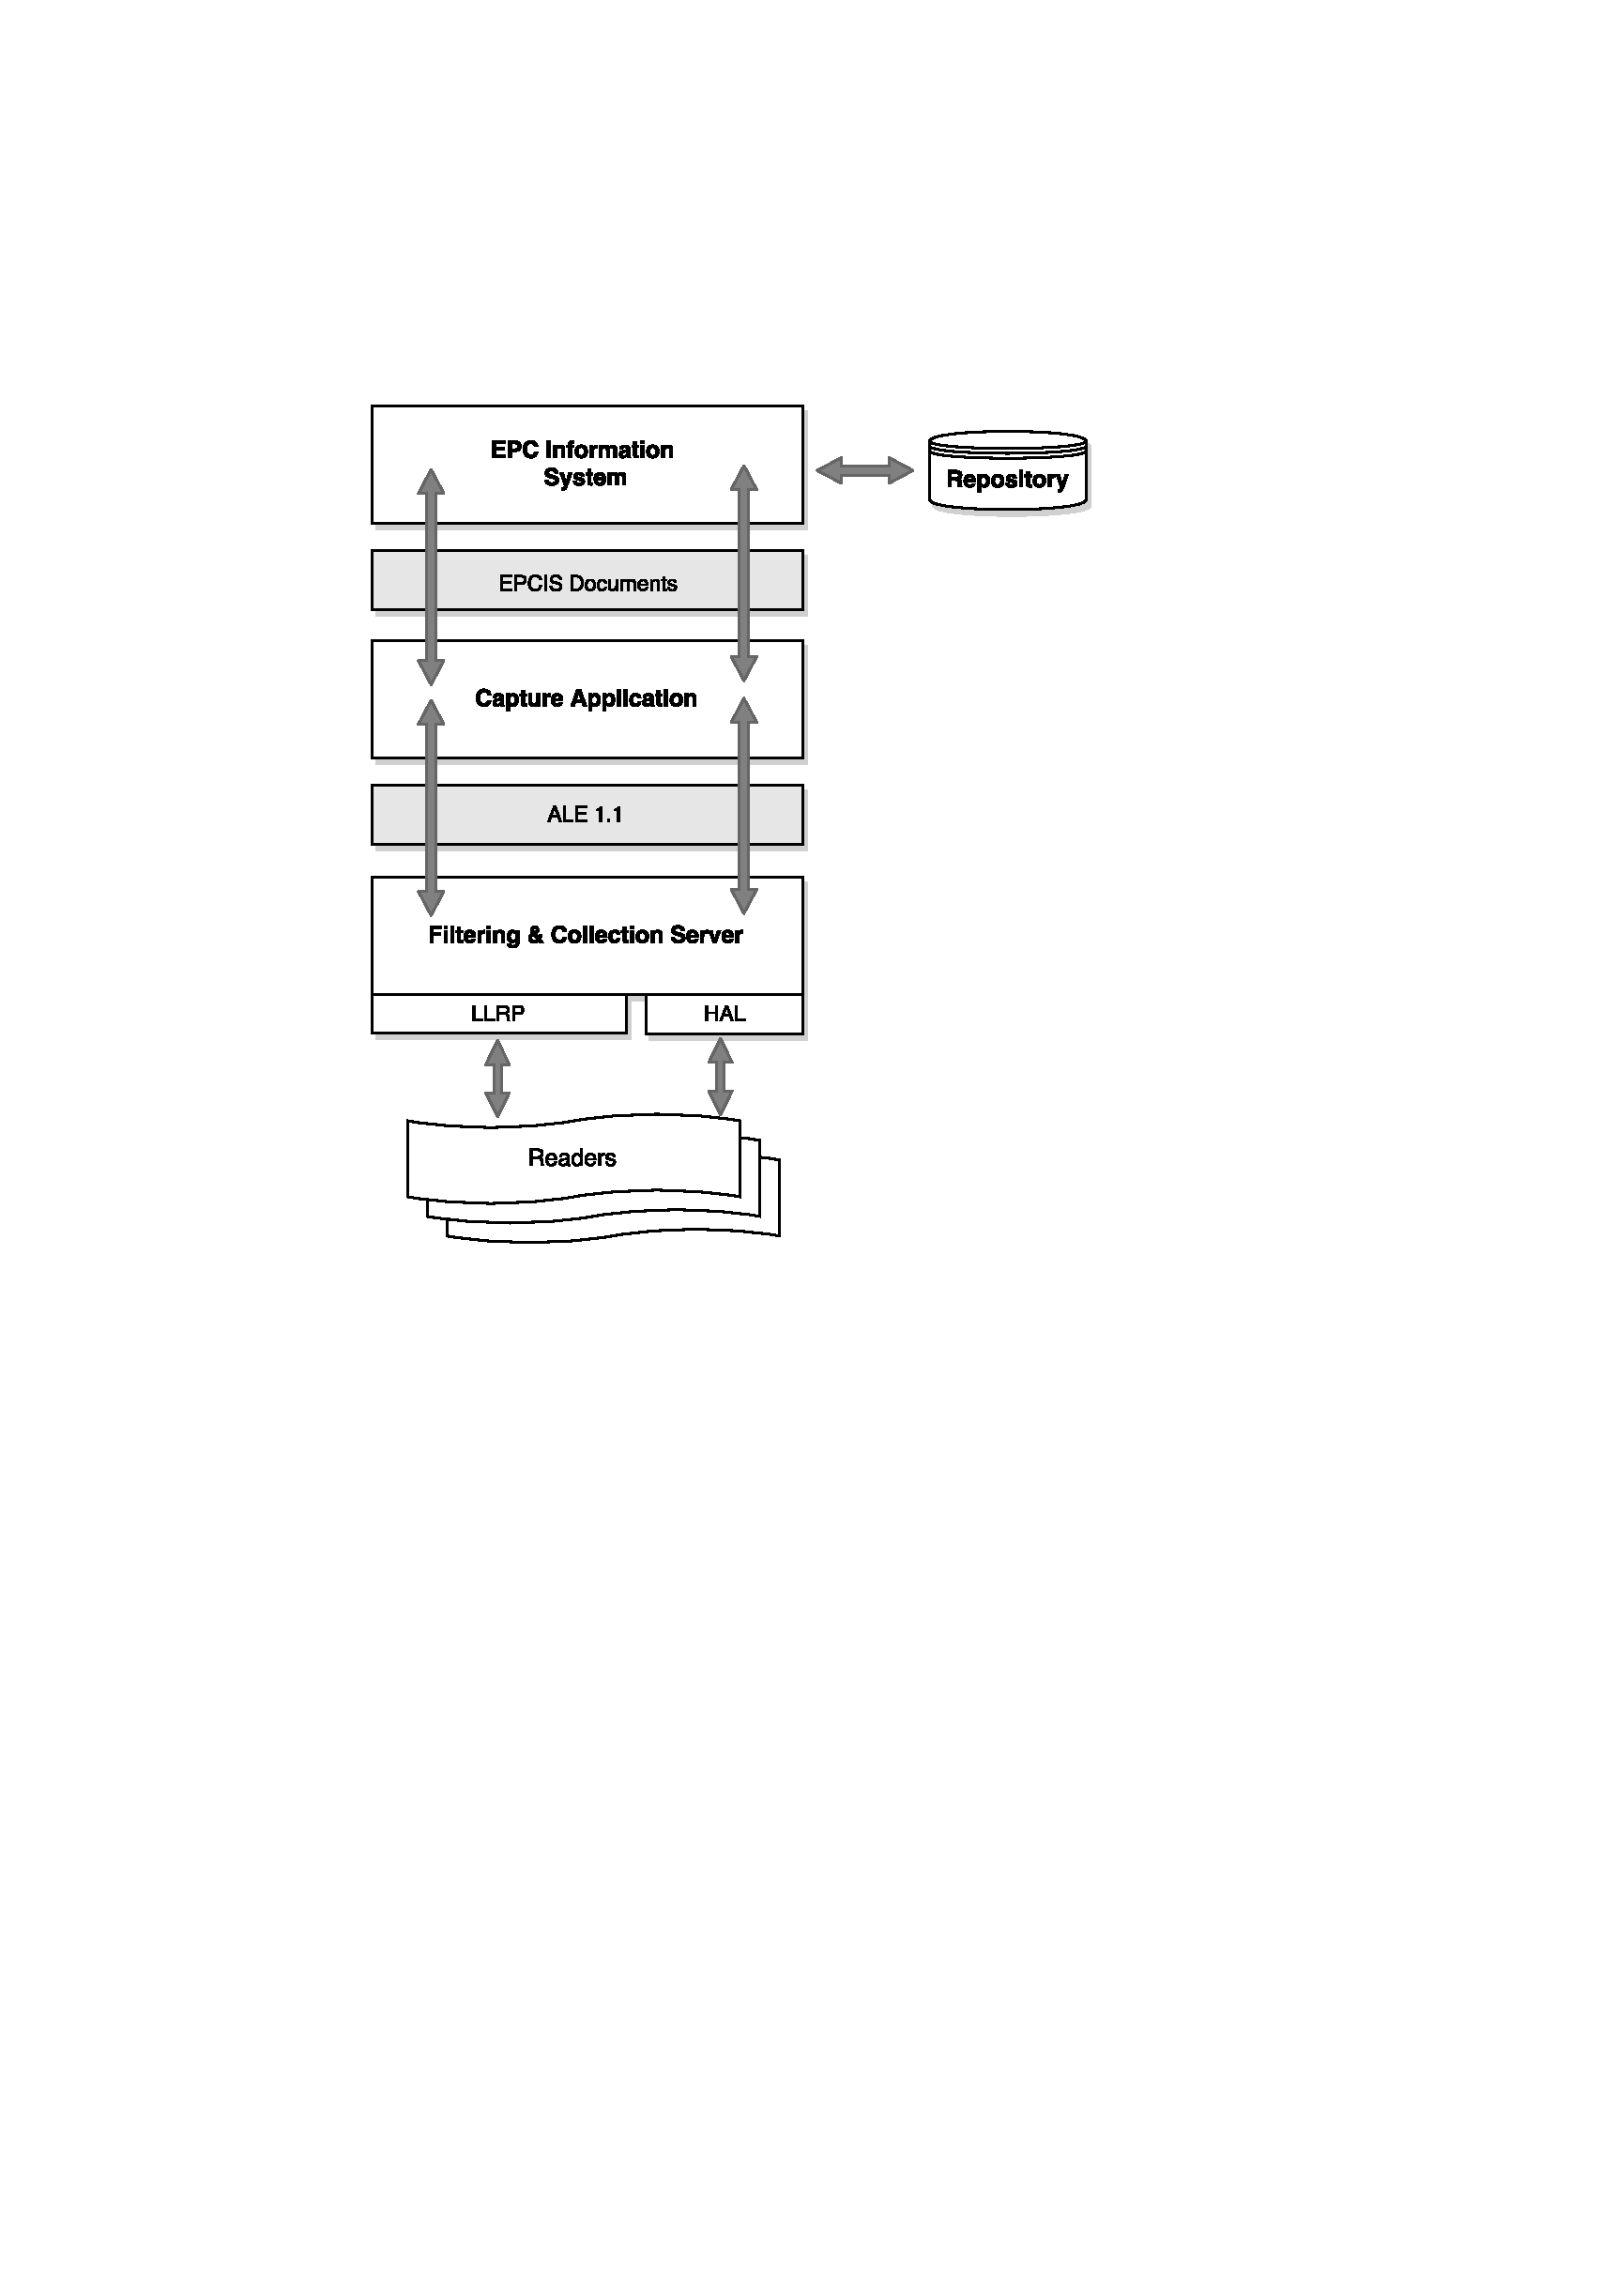
\includegraphics[width=.65\textwidth]{./images/fosstrak_architecture}
  \caption[Fosstrak architecture.]{Fosstrak architecture.}
  \label{fig:fosstrak_architecture}
\end{figure}

The Fosstrak platform is composed of three modules that implements the corresponding roles in the
\gls{EPC} Network: \textit{Reader Module}, \textit{Filtering and Collection Middleware Module} and
\textit{EPCIS Module}. For our work the relevant modules of the platform are:

% Fosstrak Modules
\begin{itemize}
  % FCServer
  \item \textit{Filtering \& Collection Server} is the module responsible to filter and collect data
  from \gls{RFID} readers. To communicate with the readers, the module uses the \gls{LLRP} standard
  for \gls{LLRP} compliant readers and uses the Fosstrak \gls{HAL} for unsupported readers. The
  module internally abstracts the readers as LogicalReaders instances that are defined and configured
  through a \textit{LRSpec} document, as defined by EPCglobal. Fosstrak also implements the
  \textit{Event Cycle}, that is an interval of time during which tags are collected. The output of
  an \textit{Event Cycle} is the \textit{ECReport} document that is sent to the Capturing Application.
  % Capturing Application
  \item \textit{Capturing Application} is part of the EPCIS module. This module is responsible to
  transform the uninterpreted events received on the \textit{ECReports} into meaningful business events.
  Regarding its implementation, the Capturing Application is built on top of the Drools\footnote{\url{http://www.drools.org/}}
  engine where rules can be specified in the form of: ``when'' something happens, ``then'' do ``this''.
  Unfortunately, the rules are static and once defined they can not be updated in runtime.
  % EPCIS Repository
  \item \textit{EPCIS Repository} provides an EPCglobal-certified EPCIS Repository, which means that
  all Fosstrak EPCIS modules and interfaces are compliant with the EPCglobal standard. This module
  provides persistence for \gls{EPCIS} events. To store new events the module provides the
  \textit{capture interface} and the \textit{query interface} to retrieve historical events is provided.
  Furthermore, the module provides two EPC Network-conformant interfaces to a relational database
  (currently MySQL).
\end{itemize}
